\chapter{深度传感对照：共聚焦 / OCT / ToF}
\label{ch:10}

本章为选读。它不展开这些技术的全部细节，而是用前面各章的光学语言说明：它们各自靠什么获得深度，分辨率与量程由什么决定，以及与结构光、立体视觉的能力边界在哪里。

\section{效果}
\label{sec:ch09-effect}

读完本章，你应能：
\begin{enumerate}
  \item 说明共聚焦针孔如何实现光学层切，以及轴向分辨率与数值孔径的关系；
  \item 用第~\ref{ch:04}~章的相干长度解释 OCT 的轴向分辨率与量程；
  \item 区分脉冲 ToF 与相位（调幅连续波）ToF，写出相位 ToF 的距离公式与无模糊量程；
  \item 用一张对照表比较五类深度传感的分辨率、量程、对材料的敏感性与系统代价；
  \item 理解口内扫描常见选型背后的取舍。
\end{enumerate}

\section{原理}
\label{sec:ch09-principle}

\subsection{共聚焦：用针孔挑出焦面}

共聚焦系统把点光源聚焦到样品，再把返回光聚焦到与光源共轭的针孔上。焦面上的点回到针孔中心，全部通过；焦面外的点在针孔处是一个弥散斑，只有少部分通过。沿光轴扫描焦面（或扫描物体），记录每个横向位置的信号最大值所在深度，即得表面高度 \citep{WilsonSheppard1984}。

轴向响应宽度（层切厚度）近似
\begin{equation}
  \Delta z_{\mathrm{conf}}\sim\frac{\lambda}{\mathrm{NA}^2}
  \label{eq:ch10-conf}
\end{equation}
（常数因子依赖针孔大小、折射率与定义：理想小针孔、小 $\NA$ 时轴向响应半高宽约 $1.3\,n\lambda/\NA^2$，针孔变大则变宽；此处只作量级比较）。与第~\ref{ch:01}~章的景深同源：$\NA$ 越大，焦面外越快模糊，层切越薄。

要点：
\begin{itemize}
  \item 深度来自\emph{焦点位置}，不需要三角基线，因此可以在很窄的探头里工作，遮挡少（照明与观测同轴）。
  \item 量程由焦面扫描行程决定；精度由轴向响应宽度与 $\SNR$ 决定，峰值插值可达响应宽度的一小部分。
  \item 并行化：用针孔阵列或光栅图案配合深度扫描，可一次获得一片区域，代价是串扰与扫描时间。
  \item 半透明材料内部的散射光被针孔大量拒绝，这是共聚焦对次表面散射天然较鲁棒的原因。
\end{itemize}

\subsection{OCT：低相干干涉}

光学相干层析（OCT）把样品臂与参考臂的反射光在探测器上干涉 \citep{Huang1991OCT}。光源是宽带低相干光（第~\ref{ch:04}~章）：只有两臂光程差小于相干长度 $l_c$ 时才出现干涉条纹。因此干涉信号的包络定位了「样品中哪一深度的反射与参考臂等光程」。

对高斯谱、中心波长 $\lambda_0$、半高宽 $\Delta\lambda$ 的光源，轴向分辨率（空气中）为
\begin{equation}
  \Delta z_{\mathrm{OCT}}=\frac{2\ln2}{\pi}\,\frac{\lambda_0^{2}}{\Delta\lambda}.
  \label{eq:ch10-oct}
\end{equation}
例：$\lambda_0=840\,\mathrm{nm}$、$\Delta\lambda=50\,\mathrm{nm}$，$\Delta z\approx6.2\,\mu\mathrm{m}$；在折射率 $n$ 的介质中再除以 $n$。注意它与\emph{横向}分辨率解耦：横向由聚焦 $\NA$ 决定，轴向由光谱宽度决定。

\begin{itemize}
  \item \textbf{时域 OCT}：机械扫描参考臂长度。
  \item \textbf{频域 OCT}：参考臂固定，用光谱仪或扫频光源记录干涉光谱，傅里叶变换得到整条深度剖面。量程由光谱采样间隔决定，$z_{\max}\approx\lambda_0^2/(4\,\delta\lambda)$（$\delta\lambda$ 为每个光谱采样的宽度）。
\end{itemize}
OCT 的独特能力是\emph{看进去}：给出组织内部多层界面的反射，而不仅是表面。代价是量程浅（毫米级）、需要逐点或逐线扫描、系统复杂。

\subsection{ToF：飞行时间}

\textbf{脉冲 ToF}：发出短脉冲，测量往返时间 $\Delta t$，$Z=c\Delta t/2$（本章 $c$ 为光速，不同于第~\ref{ch:01}~章的弥散圆直径）。$1\,\mathrm{mm}$ 深度对应约 $6.7\,\mathrm{ps}$ 往返时间，可见毫米级精度需要皮秒级时间分辨。

\textbf{相位 ToF（调幅连续波）}：光源强度按调制频率 $F_m$（角频率 $\omega_m=2\pi F_m$；注意：$F_m$ 是强度包络的调制频率，通常为数十兆赫兹，远低于光频 $\nu$）正弦调制。返回光相对发射光有相位延迟 $\phi_m$，则
\begin{equation}
  Z=\frac{c}{4\pi F_m}\,\phi_m,\qquad Z_{\mathrm{amb}}=\frac{c}{2F_m}.
  \label{eq:ch10-tof}
\end{equation}
$Z_{\mathrm{amb}}$ 为无模糊量程：$F_m=20\,\mathrm{MHz}$ 时约 $7.5\,\mathrm{m}$。相位通常由每像素四个相位采样求得，形式与第~\ref{ch:07}~章的四步相移完全相同 \citep{LangeSeitz2001ToF}，于是深度噪声
\[
  \sigma_Z\approx\frac{c}{4\pi F_m}\,\sigma_{\phi_m},
\]
$\sigma_{\phi_m}$ 同样反比于调制幅与 $\SNR$。这里的「条纹」不在空间而在时间上：$c/(2F_m)$ 扮演条纹周期的角色。即便 $F_m=100\,\mathrm{MHz}$，周期也有 $1.5\,\mathrm{m}$，$0.01\,\mathrm{rad}$ 相位噪声对应约 $2.4\,\mathrm{mm}$。这解释了 ToF 在近距离精细测量上的根本劣势。多频 ToF 展开相位的思路与第~\ref{ch:07}~章多频外差相同。

ToF 的典型误差：多径干扰（墙角、凹面中光经过多次反射，等价于结构光的互反射）、次表面散射造成的延迟、混合像素（边缘飞点），以及温度引起的相位漂移。

\subsection{能力边界对照}

\begin{table}[htbp]
  \centering
  \small
  \begin{tabular}{@{}p{0.10\textwidth}p{0.12\textwidth}p{0.19\textwidth}p{0.19\textwidth}p{0.22\textwidth}@{}}
    \toprule
    方式 & 深度来源 & 轴向分辨率（量级） & 量程（量级） & 主要限制 \\
    \midrule
    共聚焦 & 焦点位置 & $1$--$20\,\mu\mathrm{m}$ & $0.1$--$20\,\mathrm{mm}$ & 扫描时间、$\NA$ 与视场 \\
    OCT & 相干门 & $2$--$10\,\mu\mathrm{m}$ & $0.5$--$5\,\mathrm{mm}$ & 量程浅、逐点扫描 \\
    结构光 & 三角+相位 & $3$--$50\,\mu\mathrm{m}$ & $1$--$500\,\mathrm{mm}$ & $\MTF$、散射、遮挡 \\
    立体 & 三角+匹配 & $10\,\mu\mathrm{m}$--$1\,\mathrm{mm}$ & $1\,\mathrm{mm}$--$20\,\mathrm{m}$ & 纹理、基线 \\
    ToF & 往返时间 & $1$--$30\,\mathrm{mm}$ & $0.1$--$20\,\mathrm{m}$ & 多径、时间分辨 \\
    \bottomrule
  \end{tabular}
  \caption{深度传感方式能力边界（数量级示意，非具体产品指标）。}
  \label{tab:ch09-compare}
\end{table}

图~\ref{fig:ch10-compare} 把同样的信息画在分辨率–量程平面上。可以看到一条大致规律：\emph{深度分辨率与量程之比}大体被各自的「编码尺度」锁定——共聚焦是焦深，OCT 是相干长度，结构光是条纹周期与基线，ToF 是调制周期。

\begin{figure}[htbp]
  \centering
  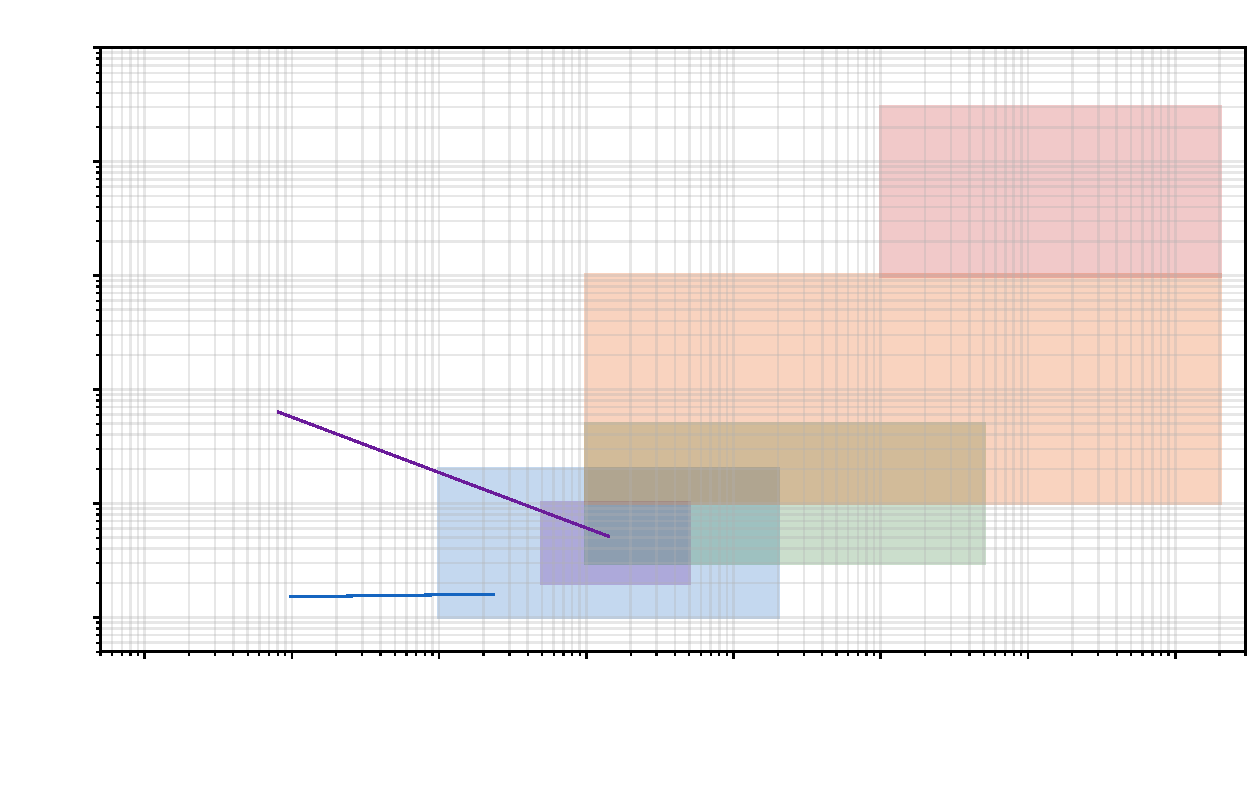
\includegraphics[width=0.85\textwidth]{fig-sensor-compare.pdf}
  \caption{各深度传感方式在分辨率–量程平面上的大致位置（概念草图，数量级示意）。}
  \label{fig:ch10-compare}
\end{figure}

\subsection{例：OCT 轴向分辨率与深度范围}

式~\eqref{eq:ch10-oct} 的轴向分辨率（高斯谱、半高全宽定义）
\[
  \Delta z=\frac{2\ln2}{\pi}\,\frac{\lambda_0^2}{\Delta\lambda}.
\]
数量级示意：$\lambda_0=840\,\mathrm{nm}$、$\Delta\lambda=50\,\mathrm{nm}$，$\Delta z\approx0.441\times0.706/0.05\approx6.2\,\mu\mathrm{m}$（空气中）。组织中光程按折射率 $n\approx1.38$ 缩短，物理深度分辨率约 $6.2/1.38\approx4.5\,\mu\mathrm{m}$。注意它只取决于光谱宽度，与物镜 $\mathrm{NA}$ 无关；横向分辨率才由 $\mathrm{NA}$ 决定。这是 OCT 能用低 $\mathrm{NA}$（大景深）同时得到微米级轴向分辨率的原因。

\textbf{频域 OCT 的深度范围。} 频域 OCT 用光谱仪记录干涉谱，深度剖面是谱的傅里叶变换。光谱仪每像素的波长间隔 $\delta\lambda_s$ 决定最大成像深度（单侧）
\[
  z_{\max}=\frac{\lambda_0^2}{4n\,\delta\lambda_s}.
\]
推导要点：干涉谱在波数 $k=2\pi/\lambda$ 上以 $\cos(2kz)$ 振荡，采样间隔 $\delta k=2\pi\delta\lambda_s/\lambda_0^2$，奈奎斯特条件 $2z\,\delta k\le\pi$。例：$2048$ 像素覆盖 $100\,\mathrm{nm}$，$\delta\lambda_s\approx0.049\,\mathrm{nm}$，空气中 $z_{\max}\approx0.706/(4\times4.9\times10^{-5})\,\mu\mathrm{m}\approx3.6\,\mathrm{mm}$。深度范围与分辨率共用同一组光谱像素：像素数固定时，覆盖更宽光谱（分辨率更好）就意味着 $\delta\lambda_s$ 更大、深度更浅。此外，光谱仪本身的有限分辨率使信号随深度衰减（称为滚降），实际可用深度短于 $z_{\max}$。

\subsection{例：共聚焦层析厚度}

按正文针孔足够小、$\mathrm{NA}$ 不大时的近似，轴向层析厚度约 $1.3\,n\lambda/\mathrm{NA}^2$。$\mathrm{NA}=0.3$、$\lambda=0.45\,\mu\mathrm{m}$、空气中：$1.3\times0.45/0.09\approx6.5\,\mu\mathrm{m}$。$\mathrm{NA}$ 减半到 $0.15$，层析厚度变为四倍约 $26\,\mu\mathrm{m}$。与 OCT 对比：共聚焦的轴向分辨率由 $\mathrm{NA}^2$ 决定，要微米级就要大 $\mathrm{NA}$，于是工作距离短、视场小、需要轴向扫描；口内共聚焦方案用平行多点阵列与轴向扫描换取视场，这是它与相移结构光在帧数与机械复杂度上的主要差别。

\subsection{例：ToF 的多径与多频}

本章已算过 $F_m=100\,\mathrm{MHz}$ 时无歧义距离 $1.5\,\mathrm{m}$ 与相位噪声对应的距离噪声。这里补两个系统项。

\textbf{多径。} 像素同时收到直接回波（幅值 $1$）与经墙角等二次反射的回波（幅值 $\beta$），后者往返总路程多出 $\Delta L$。连续波 ToF 的相位正比于往返路程，二者相位差 $\Delta\phi=2\pi F_m\Delta L/c$（此处 $c$ 为光速）。与混合像素同理，合成相位
\[
  \delta\phi=\operatorname{atan2}\bigl(\beta\sin\Delta\phi,\ 1+\beta\cos\Delta\phi\bigr).
\]
数量级示意：$\beta=0.2$、$\Delta L=0.3\,\mathrm{m}$，$\Delta\phi\approx0.63\,\mathrm{rad}$，$\delta\phi\approx0.10\,\mathrm{rad}$，换算距离 $c\,\delta\phi/(4\pi F_m)\approx2.4\,\mathrm{cm}$，比典型随机噪声大一个数量级，且总是使距离偏远。多径误差随 $F_m$ 变化（$\Delta\phi$ 正比于 $F_m$），这正是多频测量能识别多径的依据。

\textbf{多频去歧义。} 用 $80\,\mathrm{MHz}$ 与 $100\,\mathrm{MHz}$ 两个频率，二者公约数 $20\,\mathrm{MHz}$，组合后无歧义距离 $c/(2\times20\,\mathrm{MHz})=7.5\,\mathrm{m}$。逻辑与第~\ref{ch:07}~章外差完全相同，噪声放大与跳级风险也同理。

\section{限度}
\label{sec:ch09-limits}

\begin{itemize}
  \item 式~\eqref{eq:ch10-conf}、\eqref{eq:ch10-oct} 的常数因子依赖定义（半高宽、针孔尺寸、谱形），只能做量级比较。
  \item 对照表忽略了速度、成本、体积与安全（激光功率）等维度，它们往往决定实际选型。
  \item 介质折射率改变光程：OCT 与 ToF 测得的是光程而非几何距离；半透明材料中共聚焦与结构光也会受到影响。
  \item 本章不涉及光度立体、焦点堆栈（depth from focus）等其他方法，它们与共聚焦或立体的原理相近。
\end{itemize}

\section{对象}
\label{sec:ch09-object}

\textbf{口内扫描常见选型（数量级示意）。} 口内场景的约束是：工作距十余毫米、深度范围数毫米到十余毫米、探头狭小、手持移动、表面湿润且半透明、精度目标数十微米。
\begin{itemize}
  \item \textbf{结构光}（相机+投影或多相机+条纹）：帧率高，单帧覆盖面积大，便于拼接；短板是散射与高反（第~\ref{ch:07}~章），以及基线受探头尺寸限制（第~\ref{ch:08}~章）。
  \item \textbf{并行共聚焦}：同轴、无遮挡、对散射较鲁棒，适合深窄的龈沟与邻面；但需要焦面扫描，单帧时间较长，对运动敏感，探头光学更复杂。
  \item \textbf{OCT}：能看到釉质下的结构（龋损、修复体界面），研究价值大；作为全牙弓表面扫描，量程与速度不足。
  \item \textbf{ToF}：精度远不够口内要求，主要见于房间尺度或人体尺度的测量。
\end{itemize}
不同产品的取舍差异主要在：用多少帧换精度、用什么方式对付散射与高反、探头允许的基线与景深。

\subsection{例：用数字排除不合适的模态}

以口扫的典型要求（深度噪声约 $10\,\mu\mathrm{m}$ 以内、工作距离十几毫米、视场十几毫米）为基准，把本章的例子放在一起比较，数量级示意：
\begin{itemize}
  \item \textbf{连续波 ToF}：$F_m=100\,\mathrm{MHz}$、相位噪声 $0.01\,\mathrm{rad}$ 时距离噪声约 $2.4\,\mathrm{mm}$，与要求差两个多数量级；要降到 $10\,\mu\mathrm{m}$，需要相位噪声 $4\times10^{-5}\,\mathrm{rad}$ 或调制频率高两个数量级，都不现实。排除。
  \item \textbf{OCT}：轴向分辨率约 $5\,\mu\mathrm{m}$ 满足要求，但频域 OCT 单次深度范围几毫米，口内曲面高差可达十几毫米，需要额外的深度追踪；且逐点或逐线扫描使得覆盖十几毫米视场的速度受限。更适合需要看表层下结构（如龋损、牙周组织）的场合。
  \item \textbf{共聚焦}：层析厚度约 $20\,\mu\mathrm{m}$ 时需 $\mathrm{NA}\approx0.17$，覆盖 $15\,\mathrm{mm}$ 深度需上千个轴向位置；可行，但代价在扫描机构与帧率上。
  \item \textbf{相移结构光}：第~\ref{ch:00}~章走查得单帧随机噪声约 $1\,\mu\mathrm{m}$，主要风险在系统项（伽马、运动、标定）。
\end{itemize}
这种比较的意义在于先用数量级排除，再对剩下的候选做细致的误差预算，而不是比较各模态的「优缺点」列表。

\section*{本章收束}
共聚焦用焦点，OCT 用相干门，ToF 用往返时间，结构光与立体用三角。每种方法都有一个「编码尺度」，分辨率是这个尺度的一小部分，量程是它的若干倍。相位 ToF 与相移结构光在数学上同构，只是一个在时间上、一个在空间上编码。口内扫描以结构光与并行共聚焦为主，取舍落在速度、散射鲁棒性与探头尺寸上。

\section{习题}
\label{sec:ch09-exercises}

\begin{enumerate}
  \item \textbf{（计算）} 共聚焦物镜 $\NA=0.3$、$\lambda=488\,\mathrm{nm}$，估算层切厚度量级。若改为 $\NA=0.1$ 呢？对口内全牙扫描意味着什么？
  \item \textbf{（计算）} OCT 光源 $\lambda_0=1300\,\mathrm{nm}$、$\Delta\lambda=100\,\mathrm{nm}$，求空气中与牙釉质（$n\approx1.6$）中的轴向分辨率。
  \item \textbf{（计算）} 相位 ToF $F_m=60\,\mathrm{MHz}$，求无模糊量程；若相位噪声 $0.005\,\mathrm{rad}$，深度噪声多少？与口内精度目标对比。
  \item \textbf{（重建场景）} 在深而窄的龈沟中，结构光扫描缺失严重而共聚焦扫描较完整。从光路几何解释。
  \item \textbf{（重建场景）} ToF 相机拍摄墙角时，角落深度系统性偏大且角落被「磨圆」。原因是什么？它与结构光中的哪种误差同源？
  \item \textbf{（设计）} 若要检测修复体边缘下方的微小间隙（数十微米、位于表面下方），应考虑哪种方法？说明理由与代价。
  \item \textbf{（推导）} 从频域 OCT 的干涉谱 $\cos(2kz)$ 与波数采样间隔出发，推导 $z_{\max}=\lambda_0^2/(4n\,\delta\lambda_s)$。
  \item \textbf{（计算）} 中心波长 $1310\,\mathrm{nm}$、带宽 $100\,\mathrm{nm}$ 的 OCT，求空气与组织（$n=1.38$）中的轴向分辨率，并与正文 $840\,\mathrm{nm}$ 系统比较。
  \item \textbf{（口扫场景）} 若要用共聚焦方式在 $\lambda=0.45\,\mu\mathrm{m}$ 下得到 $20\,\mu\mathrm{m}$ 层析厚度，$\mathrm{NA}$ 应取多少？若口内需要 $15\,\mathrm{mm}$ 深度范围，按层析厚度的一半为轴向步距，需要多少个轴向位置？
  \item \textbf{（医学重建）} 正文多径例中，若改用 $F_m=20\,\mathrm{MHz}$ 测同一场景，$\delta\phi$ 与距离误差各为多少？据此说明多频如何用于识别多径。
  \item \textbf{（C++/CUDA 实践）} 频域 OCT 重建需要把光谱从等波长间隔重采样到等波数间隔再做 FFT。说明为什么必须重采样，并给出 GPU 上的实现要点（查表插值、批量 FFT）。
\end{enumerate}

\section{习题讲解}
\label{sec:ch09-solutions}

\begin{enumerate}
  \item $\lambda/\NA^2\approx0.488/0.09\approx5.4\,\mu\mathrm{m}$；$\NA=0.1$ 时约 $49\,\mu\mathrm{m}$。$\NA$ 大层切薄、精度高，但视场与景深小，需要更长的扫描行程与时间；口内常取中等 $\NA$ 折中。
  \item $\Delta z=0.44\times1300^2/100\,\mathrm{nm}\approx7.5\,\mu\mathrm{m}$（空气），釉质中约 $4.7\,\mu\mathrm{m}$。
  \item $Z_{\mathrm{amb}}=c/(2F_m)=2.5\,\mathrm{m}$；$\sigma_Z=c\sigma_{\phi_m}/(4\pi F_m)\approx3\times10^8\times0.005/(4\pi\times6\times10^7)\approx2\,\mathrm{mm}$，比口内目标大约两个数量级。
  \item 结构光需要投影与相机两个方向都能看到沟底，基线带来阴影与遮挡；共聚焦照明与观测同轴，只要一个方向能看到即可。
  \item 多径干扰：光在两面墙之间多次反射后返回，路径更长，相位延迟偏大。与结构光中的互反射同源，都违反「每像素只接收一次直接反射」的假设。
  \item OCT：能分辨表面以下的界面，轴向分辨率数微米。代价：量程浅、扫描慢、系统复杂，需与表面扫描配合使用。
  \item 干涉项 $\cos(2nkz)$ 在 $k$ 上的周期为 $\pi/(nz)$。$\lambda$ 等间隔 $\delta\lambda_s$ 对应 $\delta k\approx2\pi\delta\lambda_s/\lambda_0^2$。每个周期至少两个采样：$\delta k\le\pi/(2nz)$，得 $z\le\pi/(2n\delta k)=\lambda_0^2/(4n\delta\lambda_s)$。
  \item 空气中 $\Delta z=0.441\times1.716/0.1\approx7.6\,\mu\mathrm{m}$，组织中约 $5.5\,\mu\mathrm{m}$。比 $840\,\mathrm{nm}$/$50\,\mathrm{nm}$ 系统略差；长波长的好处是组织散射更弱、穿透更深。
  \item $\mathrm{NA}^2=1.3\times0.45/20\approx0.029$，$\mathrm{NA}\approx0.17$。步距 $10\,\mu\mathrm{m}$，$15\,\mathrm{mm}$ 需 $1500$ 个轴向位置，远多于相移结构光的帧数，说明共聚焦方案需要高速轴向扫描与高帧率传感器。
  \item $\Delta\phi=2\pi\times0.02\times0.3/0.3\approx0.126\,\mathrm{rad}$，$\delta\phi=\operatorname{atan2}(0.2\times0.125,1+0.2\times0.992)\approx0.021\,\mathrm{rad}$，距离误差 $3\times10^8\times0.021/(4\pi\times2\times10^7)\approx2.5\,\mathrm{cm}$。两频的距离偏差随 $\Delta L$ 与频率的关系不同（一般不相等）；若两频测得的距离在去歧义后不一致且超出噪声，就提示多径。本例数字接近，说明单凭两个频率不总能分辨，常需更多频率拟合两分量模型。
  \item 光谱仪按 $\lambda$ 近似等间隔采样，而深度与 $k$ 成傅里叶对；不重采样直接 FFT，深层信号的频率随 $k$ 漂移（啁啾），轴向峰展宽，分辨率随深度恶化。GPU 实现：预计算每个输出 $k$ 样本对应的输入像素索引与插值权重（查找表，常量或纹理内存）；每线程算一个输出样本；对所有 A 扫描用批量 FFT（如 cuFFT 的 batched 接口）一次完成；最后取模、对数压缩。
\end{enumerate}
